% Options for packages loaded elsewhere
\PassOptionsToPackage{unicode}{hyperref}
\PassOptionsToPackage{hyphens}{url}
%
\documentclass[
]{article}
\title{Homework1}
\author{Tara Dolan}
\date{9/22/2023}

\usepackage{amsmath,amssymb}
\usepackage{lmodern}
\usepackage{iftex}
\ifPDFTeX
  \usepackage[T1]{fontenc}
  \usepackage[utf8]{inputenc}
  \usepackage{textcomp} % provide euro and other symbols
\else % if luatex or xetex
  \usepackage{unicode-math}
  \defaultfontfeatures{Scale=MatchLowercase}
  \defaultfontfeatures[\rmfamily]{Ligatures=TeX,Scale=1}
\fi
% Use upquote if available, for straight quotes in verbatim environments
\IfFileExists{upquote.sty}{\usepackage{upquote}}{}
\IfFileExists{microtype.sty}{% use microtype if available
  \usepackage[]{microtype}
  \UseMicrotypeSet[protrusion]{basicmath} % disable protrusion for tt fonts
}{}
\makeatletter
\@ifundefined{KOMAClassName}{% if non-KOMA class
  \IfFileExists{parskip.sty}{%
    \usepackage{parskip}
  }{% else
    \setlength{\parindent}{0pt}
    \setlength{\parskip}{6pt plus 2pt minus 1pt}}
}{% if KOMA class
  \KOMAoptions{parskip=half}}
\makeatother
\usepackage{xcolor}
\IfFileExists{xurl.sty}{\usepackage{xurl}}{} % add URL line breaks if available
\IfFileExists{bookmark.sty}{\usepackage{bookmark}}{\usepackage{hyperref}}
\hypersetup{
  pdftitle={Homework1},
  pdfauthor={Tara Dolan},
  hidelinks,
  pdfcreator={LaTeX via pandoc}}
\urlstyle{same} % disable monospaced font for URLs
\usepackage[margin=1in]{geometry}
\usepackage{color}
\usepackage{fancyvrb}
\newcommand{\VerbBar}{|}
\newcommand{\VERB}{\Verb[commandchars=\\\{\}]}
\DefineVerbatimEnvironment{Highlighting}{Verbatim}{commandchars=\\\{\}}
% Add ',fontsize=\small' for more characters per line
\usepackage{framed}
\definecolor{shadecolor}{RGB}{248,248,248}
\newenvironment{Shaded}{\begin{snugshade}}{\end{snugshade}}
\newcommand{\AlertTok}[1]{\textcolor[rgb]{0.94,0.16,0.16}{#1}}
\newcommand{\AnnotationTok}[1]{\textcolor[rgb]{0.56,0.35,0.01}{\textbf{\textit{#1}}}}
\newcommand{\AttributeTok}[1]{\textcolor[rgb]{0.77,0.63,0.00}{#1}}
\newcommand{\BaseNTok}[1]{\textcolor[rgb]{0.00,0.00,0.81}{#1}}
\newcommand{\BuiltInTok}[1]{#1}
\newcommand{\CharTok}[1]{\textcolor[rgb]{0.31,0.60,0.02}{#1}}
\newcommand{\CommentTok}[1]{\textcolor[rgb]{0.56,0.35,0.01}{\textit{#1}}}
\newcommand{\CommentVarTok}[1]{\textcolor[rgb]{0.56,0.35,0.01}{\textbf{\textit{#1}}}}
\newcommand{\ConstantTok}[1]{\textcolor[rgb]{0.00,0.00,0.00}{#1}}
\newcommand{\ControlFlowTok}[1]{\textcolor[rgb]{0.13,0.29,0.53}{\textbf{#1}}}
\newcommand{\DataTypeTok}[1]{\textcolor[rgb]{0.13,0.29,0.53}{#1}}
\newcommand{\DecValTok}[1]{\textcolor[rgb]{0.00,0.00,0.81}{#1}}
\newcommand{\DocumentationTok}[1]{\textcolor[rgb]{0.56,0.35,0.01}{\textbf{\textit{#1}}}}
\newcommand{\ErrorTok}[1]{\textcolor[rgb]{0.64,0.00,0.00}{\textbf{#1}}}
\newcommand{\ExtensionTok}[1]{#1}
\newcommand{\FloatTok}[1]{\textcolor[rgb]{0.00,0.00,0.81}{#1}}
\newcommand{\FunctionTok}[1]{\textcolor[rgb]{0.00,0.00,0.00}{#1}}
\newcommand{\ImportTok}[1]{#1}
\newcommand{\InformationTok}[1]{\textcolor[rgb]{0.56,0.35,0.01}{\textbf{\textit{#1}}}}
\newcommand{\KeywordTok}[1]{\textcolor[rgb]{0.13,0.29,0.53}{\textbf{#1}}}
\newcommand{\NormalTok}[1]{#1}
\newcommand{\OperatorTok}[1]{\textcolor[rgb]{0.81,0.36,0.00}{\textbf{#1}}}
\newcommand{\OtherTok}[1]{\textcolor[rgb]{0.56,0.35,0.01}{#1}}
\newcommand{\PreprocessorTok}[1]{\textcolor[rgb]{0.56,0.35,0.01}{\textit{#1}}}
\newcommand{\RegionMarkerTok}[1]{#1}
\newcommand{\SpecialCharTok}[1]{\textcolor[rgb]{0.00,0.00,0.00}{#1}}
\newcommand{\SpecialStringTok}[1]{\textcolor[rgb]{0.31,0.60,0.02}{#1}}
\newcommand{\StringTok}[1]{\textcolor[rgb]{0.31,0.60,0.02}{#1}}
\newcommand{\VariableTok}[1]{\textcolor[rgb]{0.00,0.00,0.00}{#1}}
\newcommand{\VerbatimStringTok}[1]{\textcolor[rgb]{0.31,0.60,0.02}{#1}}
\newcommand{\WarningTok}[1]{\textcolor[rgb]{0.56,0.35,0.01}{\textbf{\textit{#1}}}}
\usepackage{graphicx}
\makeatletter
\def\maxwidth{\ifdim\Gin@nat@width>\linewidth\linewidth\else\Gin@nat@width\fi}
\def\maxheight{\ifdim\Gin@nat@height>\textheight\textheight\else\Gin@nat@height\fi}
\makeatother
% Scale images if necessary, so that they will not overflow the page
% margins by default, and it is still possible to overwrite the defaults
% using explicit options in \includegraphics[width, height, ...]{}
\setkeys{Gin}{width=\maxwidth,height=\maxheight,keepaspectratio}
% Set default figure placement to htbp
\makeatletter
\def\fps@figure{htbp}
\makeatother
\setlength{\emergencystretch}{3em} % prevent overfull lines
\providecommand{\tightlist}{%
  \setlength{\itemsep}{0pt}\setlength{\parskip}{0pt}}
\setcounter{secnumdepth}{-\maxdimen} % remove section numbering
\ifLuaTeX
  \usepackage{selnolig}  % disable illegal ligatures
\fi

\begin{document}
\maketitle

load required packages

\begin{Shaded}
\begin{Highlighting}[]
\NormalTok{packages }\OtherTok{\textless{}{-}}\FunctionTok{c}\NormalTok{(}\StringTok{"data.table"}\NormalTok{,}\StringTok{"fishmethods"}\NormalTok{,}\StringTok{"tidyverse"}\NormalTok{)}
\FunctionTok{lapply}\NormalTok{(packages,require,}\AttributeTok{character.only =} \ConstantTok{TRUE}\NormalTok{)}
\end{Highlighting}
\end{Shaded}

\begin{verbatim}
## Warning: package 'fishmethods' was built under R version 4.1.2
\end{verbatim}

\begin{verbatim}
## Warning in checkMatrixPackageVersion(): Package version inconsistency detected.
## TMB was built with Matrix version 1.3.4
## Current Matrix version is 1.5.1
## Please re-install 'TMB' from source using install.packages('TMB', type = 'source') or ask CRAN for a binary version of 'TMB' matching CRAN's 'Matrix' package
\end{verbatim}

\begin{verbatim}
## Warning: package 'ggplot2' was built under R version 4.1.2
\end{verbatim}

\begin{verbatim}
## [[1]]
## [1] TRUE
## 
## [[2]]
## [1] TRUE
## 
## [[3]]
## [1] TRUE
\end{verbatim}

\textbf{1.Draw a graph of the population model variables, including
relationships linking data, population variables, and parameters} \$\$
1.: data: \hat{N_t} \textbackslash{} 2.: process: N\_\{t+1\}=(1+r)N\_t +
\varepsilon \textbackslash{} 3.: parameters: N\_t, \sigma\^{}2, r
\textbackslash{} : \textbackslash{} Where,\textbackslash{} 4.
:ln(\hat{N_t}) \sim Normdist(ln(N\_t), \sigma\^{}2)

\[
There should be arrows going from \]\hat{N_t}\[ in line 1 to  \]N\_t\[ on line 4; between \]r\[ on line 2 and \]r\[ on line 3; between the observation error \]\varepsilon\[ on line 2 and the sample variance \]\sigma\^{}2\$\$
on lines 3 and 4.

\textbf{2. Reparameterize the population dynamics model so that the
numbers at time t are a function of the growth rate r and the population
size in 1978}\\
\[
N_t=N_{t=1978}(1+r)
\]

\textbf{3. Fit the population dynamics model to the available abundance
data. You can assume that the observation error variance does not change
over time and is an estimable parameter.}

\begin{Shaded}
\begin{Highlighting}[]
\CommentTok{\#data}
\NormalTok{BCBW }\OtherTok{\textless{}{-}}\FunctionTok{data.table}\NormalTok{(}\AttributeTok{Year=}\FunctionTok{c}\NormalTok{(}\DecValTok{1978}\NormalTok{,}\DecValTok{1980}\NormalTok{,}\DecValTok{1981}\NormalTok{,}\DecValTok{1982}\NormalTok{,}\DecValTok{1983}\NormalTok{,}\DecValTok{1985}\NormalTok{,}\DecValTok{1986}\NormalTok{,}\DecValTok{1987}\NormalTok{,}\DecValTok{1988}\NormalTok{,}\DecValTok{1993}\NormalTok{,}\DecValTok{2001}\NormalTok{),}
                  \AttributeTok{Number=}\FunctionTok{c}\NormalTok{(}\DecValTok{4765}\NormalTok{,}\DecValTok{3885}\NormalTok{,}\DecValTok{4467}\NormalTok{,}\DecValTok{7395}\NormalTok{,}\DecValTok{6573}\NormalTok{,}\DecValTok{5762}\NormalTok{,}\DecValTok{8917}\NormalTok{,}\DecValTok{5298}\NormalTok{,}\DecValTok{6928}\NormalTok{,}\DecValTok{8167}\NormalTok{,}\DecValTok{10545}\NormalTok{),}
                  \AttributeTok{CV=}\FunctionTok{c}\NormalTok{(}\FloatTok{0.305}\NormalTok{,}\FloatTok{0.343}\NormalTok{,}\FloatTok{0.273}\NormalTok{,}\FloatTok{0.281}\NormalTok{,}\FloatTok{0.345}\NormalTok{,}\FloatTok{0.253}\NormalTok{,}\FloatTok{0.215}\NormalTok{,}\FloatTok{0.327}\NormalTok{,}\FloatTok{0.12}\NormalTok{,}\FloatTok{0.071}\NormalTok{,}\FloatTok{0.128}\NormalTok{))  }

\CommentTok{\#We are going to linearize the model, so create a log of Nt  }
\NormalTok{BCBW }\OtherTok{\textless{}{-}} \FunctionTok{mutate}\NormalTok{(BCBW,}\AttributeTok{lnNumber=}\FunctionTok{log}\NormalTok{(Number))}
\CommentTok{\#create a log for the offset}
\NormalTok{BCBW }\OtherTok{\textless{}{-}}\FunctionTok{mutate}\NormalTok{(BCBW, }\AttributeTok{ln1978=}\FunctionTok{log}\NormalTok{(BCBW}\SpecialCharTok{$}\NormalTok{Number[BCBW}\SpecialCharTok{$}\NormalTok{Year}\SpecialCharTok{==}\StringTok{"1978"}\NormalTok{]), }\AttributeTok{n1978=}\NormalTok{BCBW}\SpecialCharTok{$}\NormalTok{Number[BCBW}\SpecialCharTok{$}\NormalTok{Year}\SpecialCharTok{==}\StringTok{"1978"}\NormalTok{])}
\CommentTok{\#make spaces in the data}
\NormalTok{Year }\OtherTok{\textless{}{-}}\FunctionTok{seq}\NormalTok{(}\DecValTok{1978}\NormalTok{,}\DecValTok{2001}\NormalTok{,}\DecValTok{1}\NormalTok{)}\SpecialCharTok{\%\textgreater{}\%}\FunctionTok{as.data.frame}\NormalTok{()}
\FunctionTok{colnames}\NormalTok{(Year)}\OtherTok{\textless{}{-}}\FunctionTok{c}\NormalTok{(}\StringTok{"Year"}\NormalTok{)}
\NormalTok{BCBW }\OtherTok{\textless{}{-}}\FunctionTok{full\_join}\NormalTok{(BCBW,Year)}\SpecialCharTok{\%\textgreater{}\%}\FunctionTok{arrange}\NormalTok{(Year)}
\end{Highlighting}
\end{Shaded}

\begin{verbatim}
## Joining, by = "Year"
\end{verbatim}

\begin{Shaded}
\begin{Highlighting}[]
\NormalTok{BCBW}\SpecialCharTok{$}\NormalTok{timestep }\OtherTok{\textless{}{-}}\FunctionTok{as.numeric}\NormalTok{(}\FunctionTok{seq}\NormalTok{(}\DecValTok{0}\NormalTok{,}\DecValTok{23}\NormalTok{,}\DecValTok{1}\NormalTok{))}

\CommentTok{\#1978 is a constant, so we want to fit data from 1979 onward}
\NormalTok{BCBW\_short }\OtherTok{\textless{}{-}}\FunctionTok{filter}\NormalTok{(BCBW, timestep }\SpecialCharTok{\textgreater{}}\DecValTok{0}\NormalTok{)}

\CommentTok{\#glm fit}
\NormalTok{glm\_fit }\OtherTok{\textless{}{-}}\FunctionTok{glm}\NormalTok{(}\FunctionTok{log}\NormalTok{(Number)}\SpecialCharTok{\textasciitilde{}}\DecValTok{0} \SpecialCharTok{+}\NormalTok{ timestep }\SpecialCharTok{+} \FunctionTok{offset}\NormalTok{(ln1978),}\AttributeTok{data=}\NormalTok{BCBW\_short)}
\FunctionTok{print}\NormalTok{(}\StringTok{"coefficients of the GLM fit"}\NormalTok{)}
\end{Highlighting}
\end{Shaded}

\begin{verbatim}
## [1] "coefficients of the GLM fit"
\end{verbatim}

\begin{Shaded}
\begin{Highlighting}[]
\FunctionTok{coef}\NormalTok{(glm\_fit)}
\end{Highlighting}
\end{Shaded}

\begin{verbatim}
##   timestep 
## 0.03643987
\end{verbatim}

\begin{Shaded}
\begin{Highlighting}[]
\CommentTok{\#linearized fit {-} not sure where the intercept comes in here. }
\NormalTok{fit\_lm }\OtherTok{\textless{}{-}} \FunctionTok{lm}\NormalTok{(BCBW\_short}\SpecialCharTok{$}\NormalTok{lnNumber }\SpecialCharTok{\textasciitilde{}}\NormalTok{ BCBW\_short}\SpecialCharTok{$}\NormalTok{timestep)}
\FunctionTok{print}\NormalTok{(}\StringTok{"coefficients of the log linear fit"}\NormalTok{)}
\end{Highlighting}
\end{Shaded}

\begin{verbatim}
## [1] "coefficients of the log linear fit"
\end{verbatim}

\begin{Shaded}
\begin{Highlighting}[]
\FunctionTok{coef}\NormalTok{(fit\_lm)}
\end{Highlighting}
\end{Shaded}

\begin{verbatim}
##         (Intercept) BCBW_short$timestep 
##          8.46561921          0.03670783
\end{verbatim}

\begin{Shaded}
\begin{Highlighting}[]
\FunctionTok{exp}\NormalTok{(fit\_lm}\SpecialCharTok{$}\NormalTok{coefficients[[}\DecValTok{1}\NormalTok{]]) }\CommentTok{\#notice that this is the 1978 number}
\end{Highlighting}
\end{Shaded}

\begin{verbatim}
## [1] 4748.667
\end{verbatim}

\begin{Shaded}
\begin{Highlighting}[]
\NormalTok{fit\_lm}\SpecialCharTok{$}\NormalTok{coefficients[[}\DecValTok{2}\NormalTok{]]}\CommentTok{\#notice that this is the same growth rate as the glm fit}
\end{Highlighting}
\end{Shaded}

\begin{verbatim}
## [1] 0.03670783
\end{verbatim}

The coefficient of the glm fit \texttt{coef(glm\_fit)} is roughly the
same as that of the lm fit \texttt{fit\_lm\$coefficients{[}{[}2{]}{]}}.
The intercept of the linear fit
\texttt{fit\_lm\$coefficients{[}{[}1{]}{]}} is (correctly) the
observation of abundance in 1978.

\textbf{4.Plot the resulting model predictions from the fitted model
along with the data, and provide comment on the fit to the data
(e.g.~via residuals, etc.)}

\begin{Shaded}
\begin{Highlighting}[]
\CommentTok{\#predict over new data on the scale of the response variable}
\NormalTok{predglm }\OtherTok{\textless{}{-}}\FunctionTok{predict}\NormalTok{(glm\_fit,}\AttributeTok{newdata=}\FunctionTok{data.frame}\NormalTok{(}\AttributeTok{timestep=}\FunctionTok{seq}\NormalTok{(}\DecValTok{0}\NormalTok{,}\DecValTok{23}\NormalTok{,}\DecValTok{1}\NormalTok{),}\AttributeTok{ln1978=}\FunctionTok{rep}\NormalTok{(}\FunctionTok{log}\NormalTok{(BCBW}\SpecialCharTok{$}\NormalTok{Number[BCBW}\SpecialCharTok{$}\NormalTok{Year}\SpecialCharTok{==}\StringTok{"1978"}\NormalTok{]))),}\AttributeTok{se.fit=}\NormalTok{T, }\AttributeTok{type=}\StringTok{"response"}\NormalTok{)}

\CommentTok{\#attach predicted values to the data frame with observed values}
\NormalTok{preds }\OtherTok{\textless{}{-}}\FunctionTok{as.data.frame}\NormalTok{(predglm)}\SpecialCharTok{\%\textgreater{}\%}\FunctionTok{rownames\_to\_column}\NormalTok{(}\AttributeTok{var=}\StringTok{"timestep"}\NormalTok{)}\SpecialCharTok{\%\textgreater{}\%}
  \FunctionTok{mutate}\NormalTok{(}\AttributeTok{timestep=}\FunctionTok{as.numeric}\NormalTok{(timestep))}
\CommentTok{\#this dataframe will not have the NA values in it}
\NormalTok{BCBW2 }\OtherTok{\textless{}{-}}\FunctionTok{full\_join}\NormalTok{(BCBW\_short, preds)}\SpecialCharTok{\%\textgreater{}\%}\FunctionTok{na.omit}\NormalTok{()}\SpecialCharTok{\%\textgreater{}\%}
  \CommentTok{\#back transform the logged predictor values to the scale of the observation data}
  \FunctionTok{mutate}\NormalTok{(}\AttributeTok{pred=}\FunctionTok{exp}\NormalTok{(fit))}
\end{Highlighting}
\end{Shaded}

\begin{verbatim}
## Joining, by = "timestep"
\end{verbatim}

\begin{Shaded}
\begin{Highlighting}[]
\CommentTok{\#plot}
\NormalTok{BCBW2}\SpecialCharTok{\%\textgreater{}\%}
  \FunctionTok{ggplot}\NormalTok{(}\FunctionTok{aes}\NormalTok{(Year,Number))}\SpecialCharTok{+}
  \FunctionTok{geom\_point}\NormalTok{()}\SpecialCharTok{+}
  \FunctionTok{geom\_line}\NormalTok{(}\FunctionTok{aes}\NormalTok{(Year, pred),}\AttributeTok{col=}\StringTok{"red"}\NormalTok{)}\SpecialCharTok{+}
  \FunctionTok{ggtitle}\NormalTok{(}\StringTok{"Abundance of BCBW with GLM fit"}\NormalTok{)}\SpecialCharTok{+}
  \FunctionTok{theme\_classic}\NormalTok{()}
\end{Highlighting}
\end{Shaded}

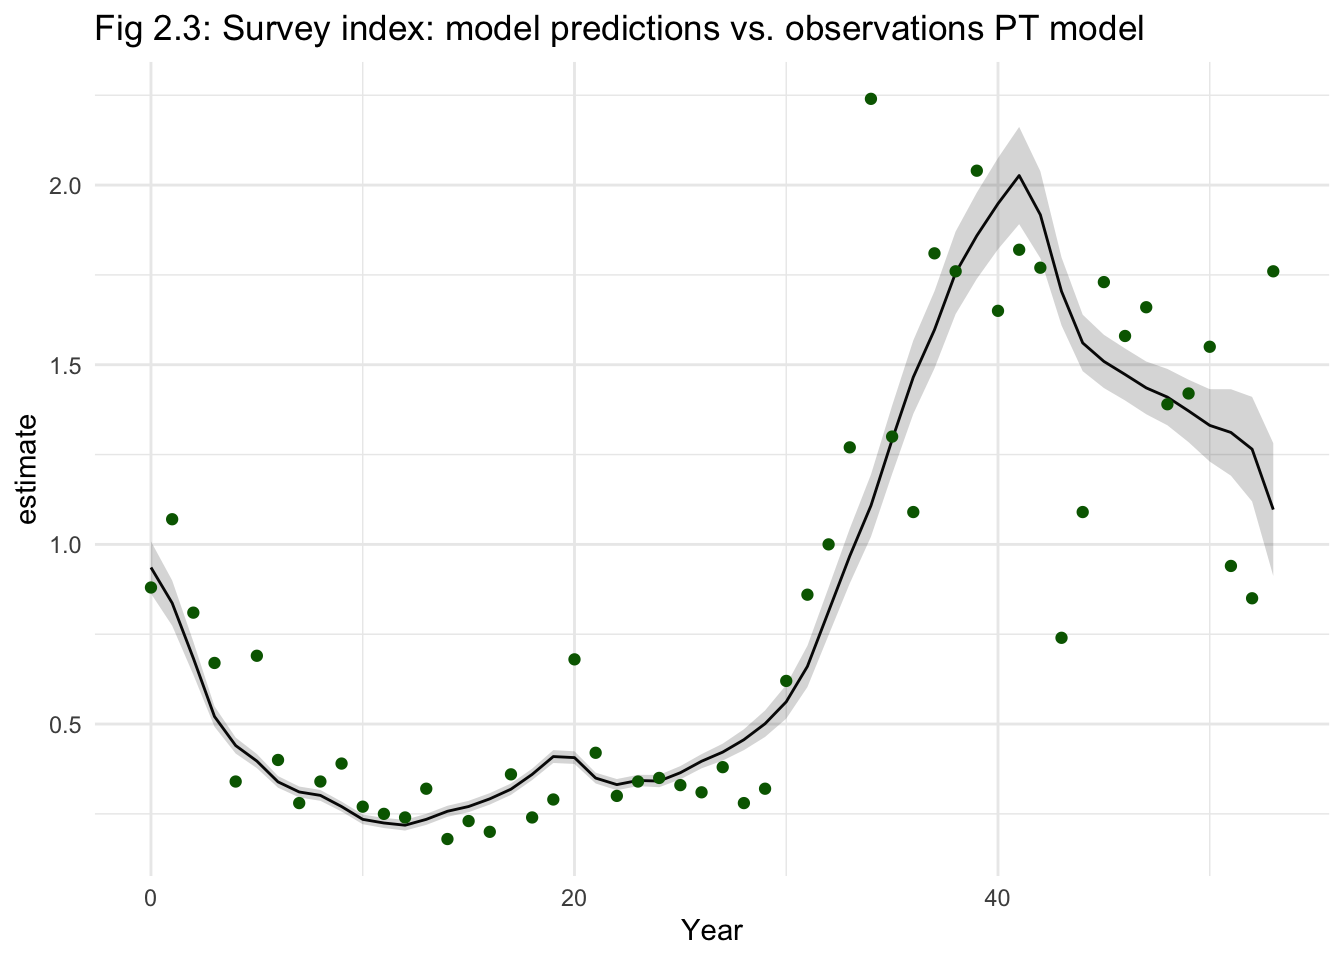
\includegraphics{hw1_tdolan_files/figure-latex/unnamed-chunk-3-1.pdf}

\begin{Shaded}
\begin{Highlighting}[]
\DocumentationTok{\#\#explore the residuals\#\#}
 \FunctionTok{plot}\NormalTok{(}\FunctionTok{density}\NormalTok{(}\FunctionTok{resid}\NormalTok{(glm\_fit, }\AttributeTok{type=}\StringTok{\textquotesingle{}pearson\textquotesingle{}}\NormalTok{)), }\AttributeTok{main=}\StringTok{"Pearson residuals"}\NormalTok{)}
\end{Highlighting}
\end{Shaded}

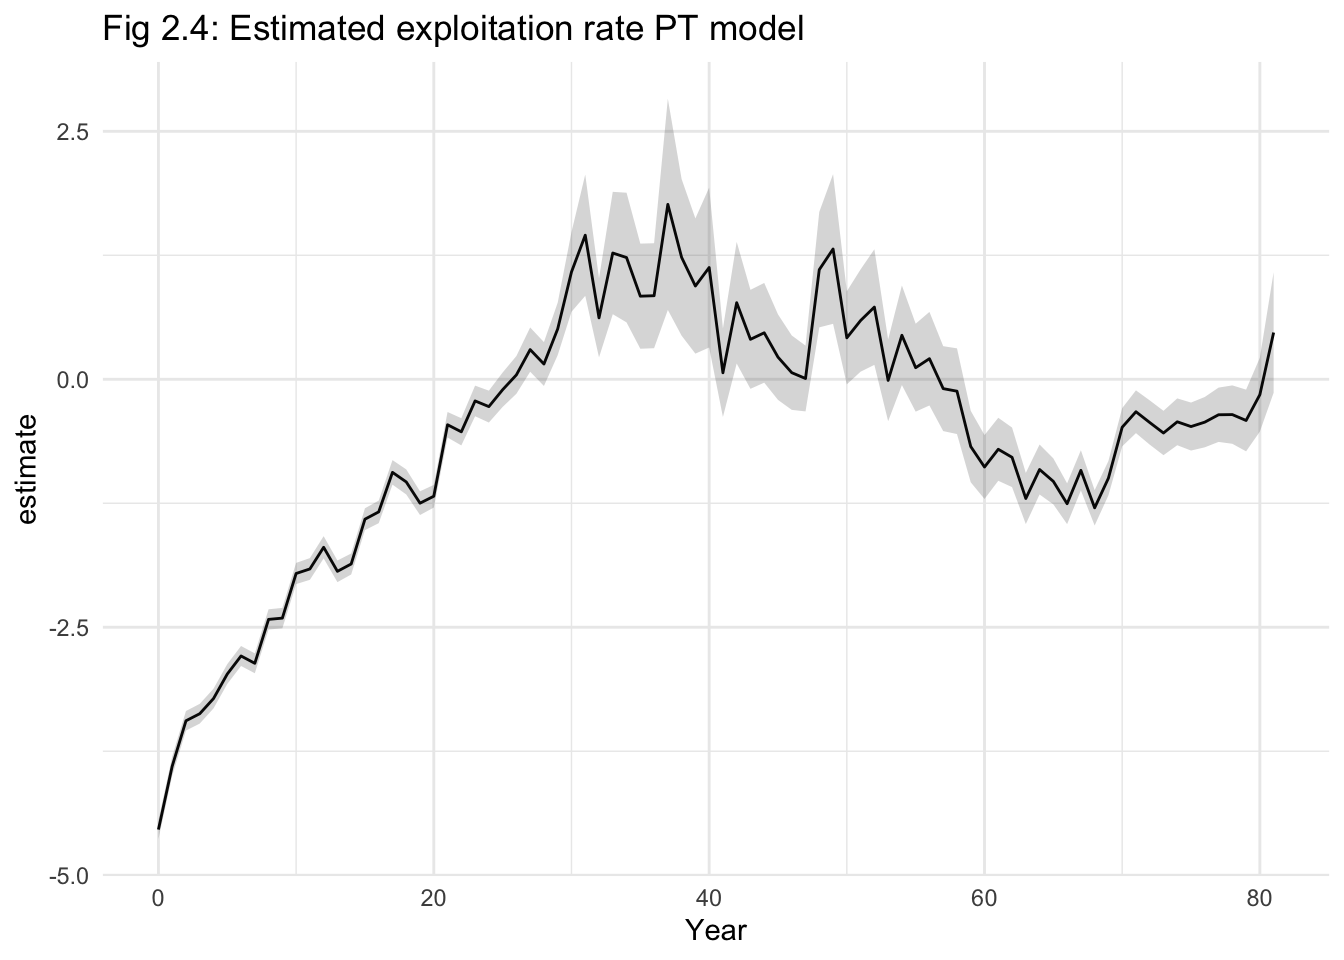
\includegraphics{hw1_tdolan_files/figure-latex/unnamed-chunk-3-2.pdf}

\begin{Shaded}
\begin{Highlighting}[]
 \FunctionTok{scatter.smooth}\NormalTok{(BCBW2}\SpecialCharTok{$}\NormalTok{Year, }\FunctionTok{rstandard}\NormalTok{(glm\_fit, }\AttributeTok{type=}\StringTok{\textquotesingle{}deviance\textquotesingle{}}\NormalTok{), }\AttributeTok{col=}\StringTok{\textquotesingle{}gray\textquotesingle{}}\NormalTok{,  }\AttributeTok{main=}\StringTok{"Pearson residuals"}\NormalTok{,}\AttributeTok{xlab=}\StringTok{"Year"}\NormalTok{,}\AttributeTok{ylab=}\StringTok{"standardized deviance residuals"}\NormalTok{)}
\end{Highlighting}
\end{Shaded}

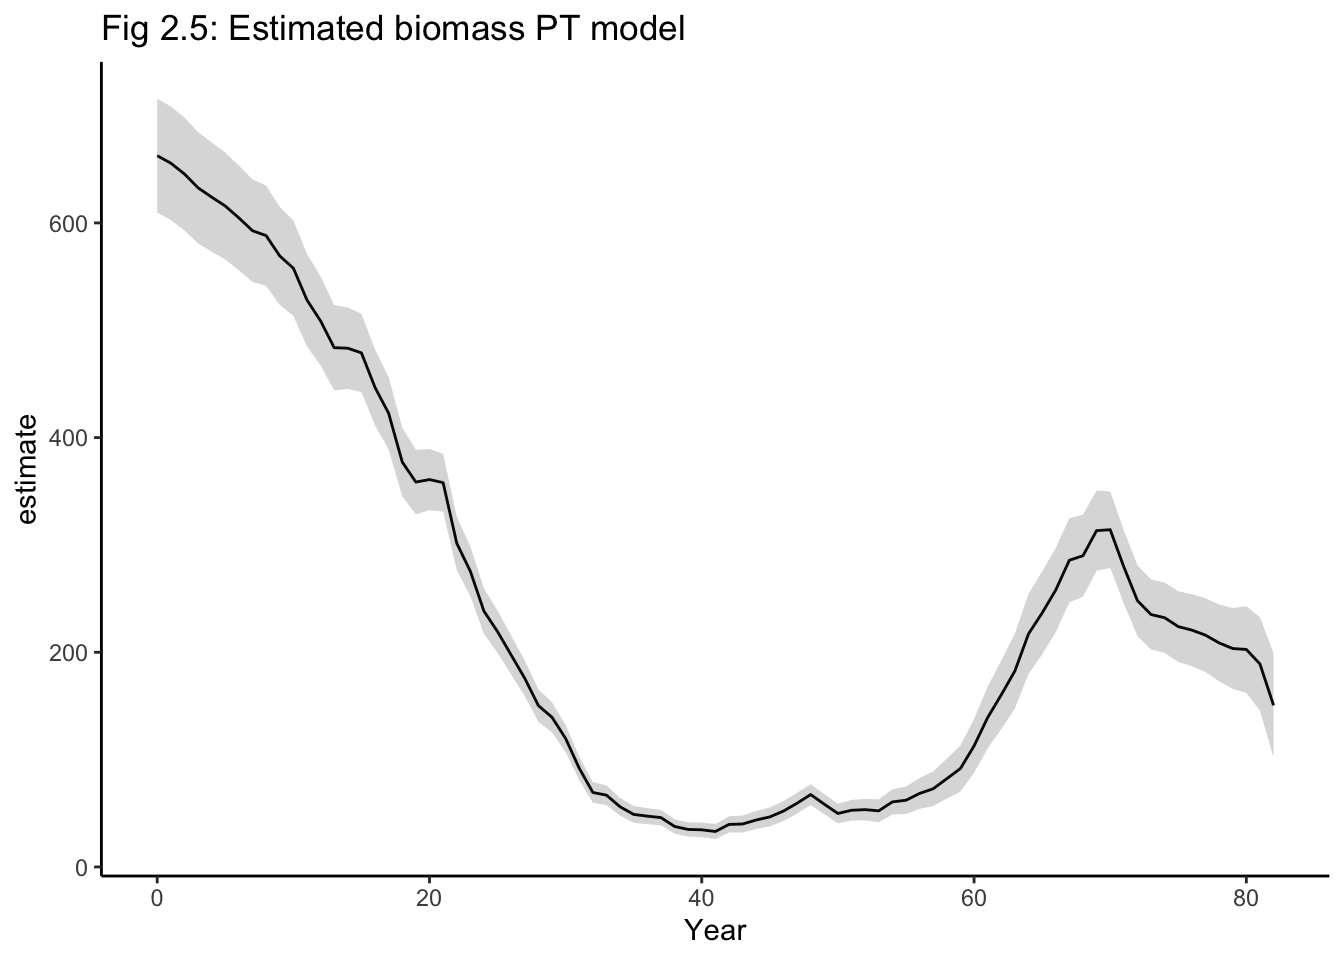
\includegraphics{hw1_tdolan_files/figure-latex/unnamed-chunk-3-3.pdf}

\begin{Shaded}
\begin{Highlighting}[]
 \FunctionTok{scatter.smooth}\NormalTok{(}\FunctionTok{predict}\NormalTok{(glm\_fit, }\AttributeTok{type=}\StringTok{\textquotesingle{}response\textquotesingle{}}\NormalTok{), }\FunctionTok{rstandard}\NormalTok{(glm\_fit, }\AttributeTok{type=}\StringTok{\textquotesingle{}deviance\textquotesingle{}}\NormalTok{),}\AttributeTok{col=}\StringTok{\textquotesingle{}gray\textquotesingle{}}\NormalTok{,}\AttributeTok{xlab=}\StringTok{"response"}\NormalTok{,}\AttributeTok{ylab=}\StringTok{"standardized deviance residuals"}\NormalTok{)}
\end{Highlighting}
\end{Shaded}

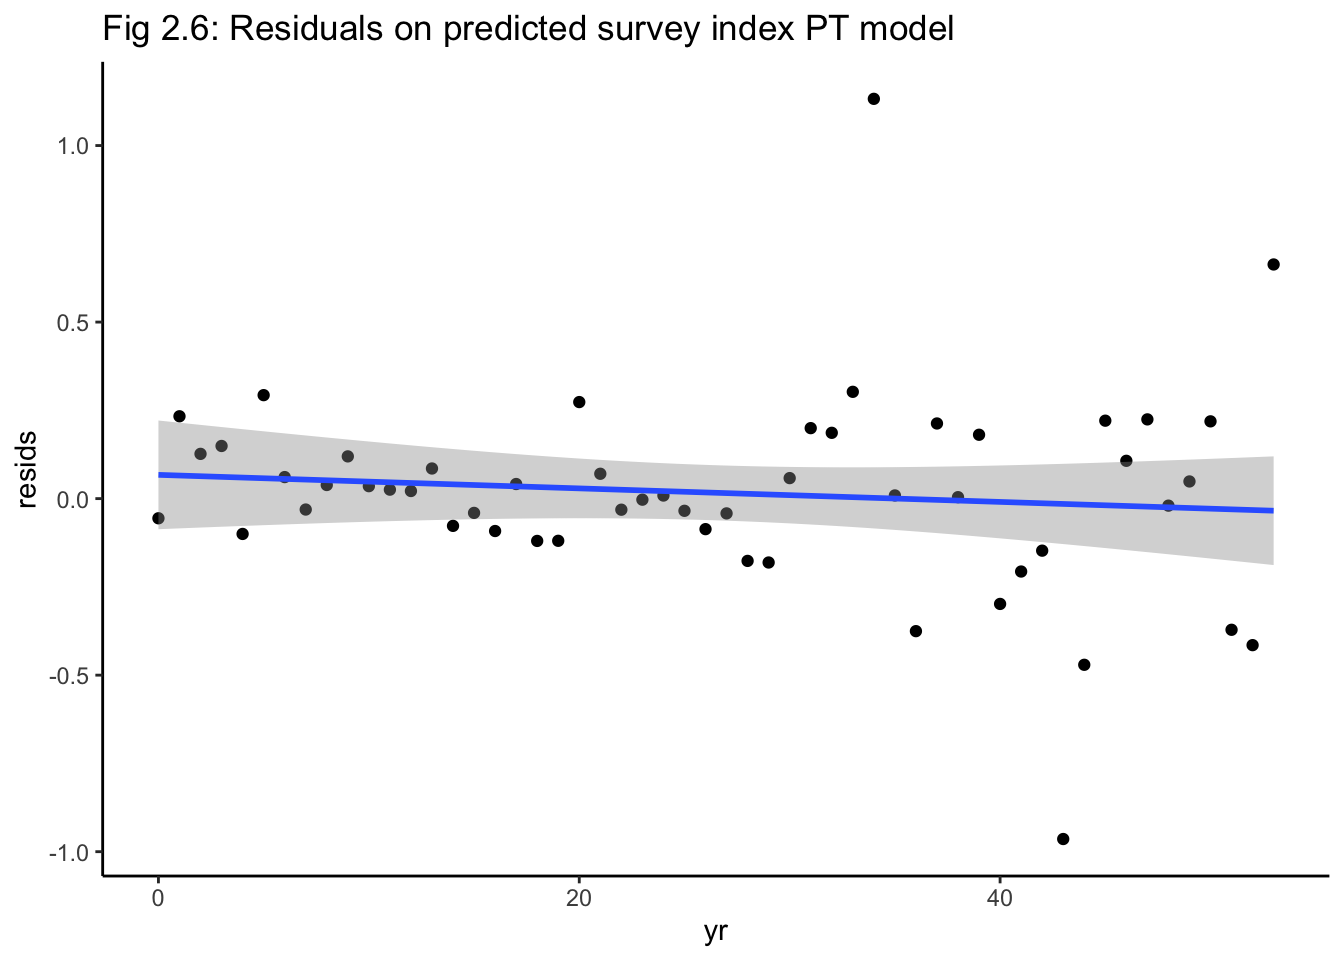
\includegraphics{hw1_tdolan_files/figure-latex/unnamed-chunk-3-4.pdf}
The data appear to be lognormally distributed. The residuals on the
lognormally fit data are approximately normally distributed. The fit
appears good but data points later in the time series likely have more
leverage because there are fewer of them.

\textbf{5. Provide an estimate for the growth rate r}\\
The coefficient for the glm represents \[
log(1+r)
\] Backtransform to get the growth rate:\\
\[
e^{(glm.coeff)}-1
\] The growth rate for the equation should be:

\begin{Shaded}
\begin{Highlighting}[]
\FunctionTok{exp}\NormalTok{(}\FunctionTok{coef}\NormalTok{(glm\_fit))}\SpecialCharTok{{-}}\DecValTok{1}
\end{Highlighting}
\end{Shaded}

\begin{verbatim}
##   timestep 
## 0.03711194
\end{verbatim}

However, we should try to plug it back in and see if it is in the
ballpark of our data \& model.

\begin{Shaded}
\begin{Highlighting}[]
\NormalTok{r}\OtherTok{=}\FunctionTok{exp}\NormalTok{(}\FunctionTok{coef}\NormalTok{(glm\_fit))}\SpecialCharTok{{-}}\DecValTok{1}
\NormalTok{BCBW2 }\OtherTok{\textless{}{-}} \FunctionTok{mutate}\NormalTok{(BCBW2, }\AttributeTok{plugin =}\NormalTok{ (}\DecValTok{1}\SpecialCharTok{+}\NormalTok{r)}\SpecialCharTok{*}\NormalTok{Number)}

\CommentTok{\#plot}
\NormalTok{BCBW2}\SpecialCharTok{\%\textgreater{}\%}
  \FunctionTok{ggplot}\NormalTok{(}\FunctionTok{aes}\NormalTok{(Year,Number))}\SpecialCharTok{+}
  \FunctionTok{geom\_point}\NormalTok{()}\SpecialCharTok{+}
  \FunctionTok{geom\_line}\NormalTok{(}\FunctionTok{aes}\NormalTok{(Year, pred),}\AttributeTok{col=}\StringTok{"red"}\NormalTok{)}\SpecialCharTok{+}
  \FunctionTok{geom\_line}\NormalTok{(}\FunctionTok{aes}\NormalTok{(Year, plugin),}\AttributeTok{col=}\StringTok{"blue"}\NormalTok{)}\SpecialCharTok{+}
  \FunctionTok{ggtitle}\NormalTok{(}\StringTok{"Abundance of BCBW with GLM fit (red) and plug in values (blue)"}\NormalTok{)}\SpecialCharTok{+}
  \FunctionTok{theme\_classic}\NormalTok{()}
\end{Highlighting}
\end{Shaded}

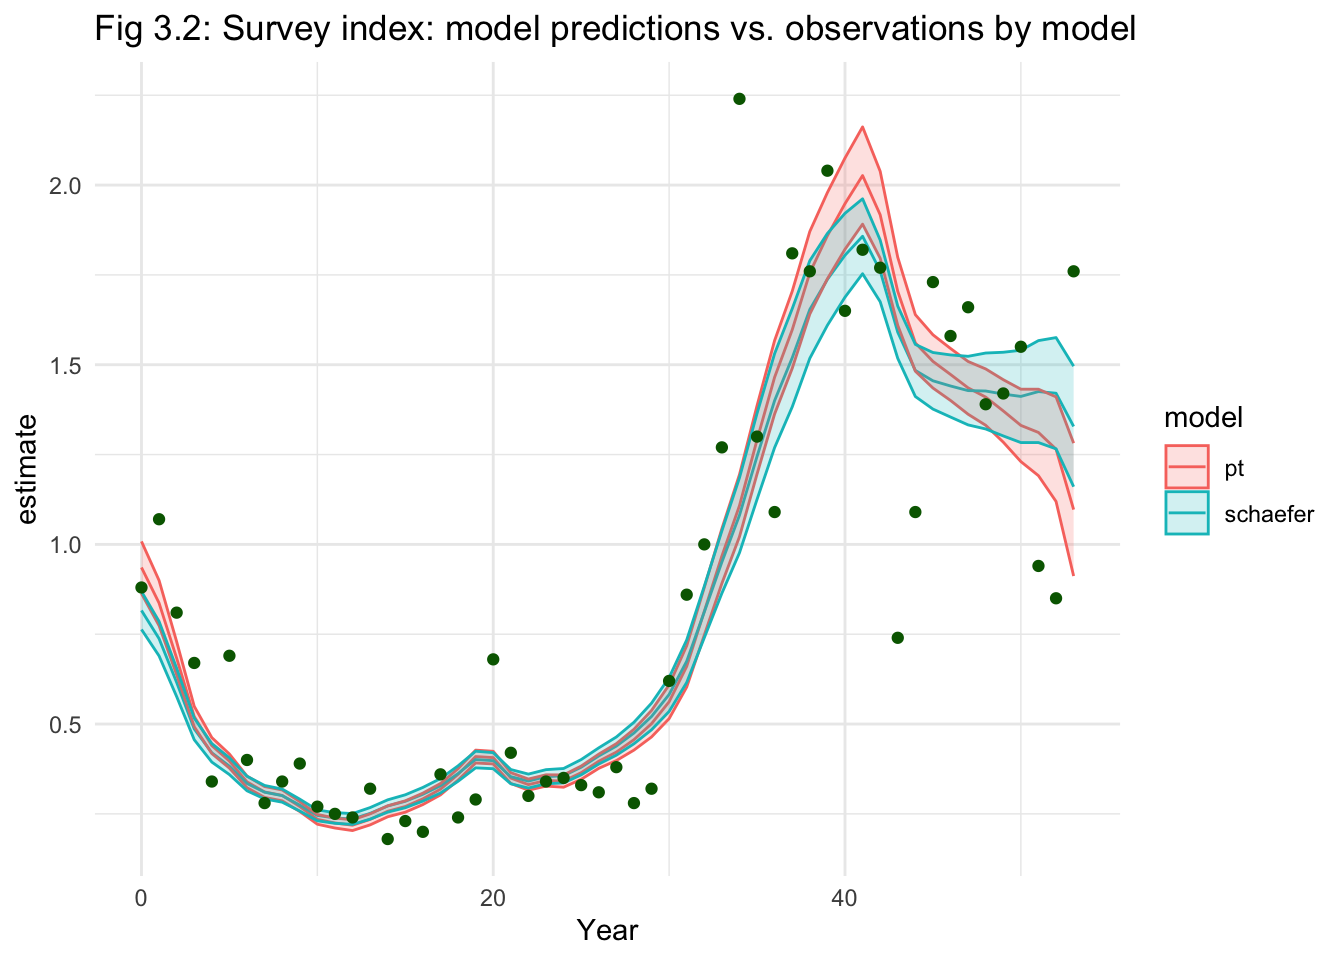
\includegraphics{hw1_tdolan_files/figure-latex/unnamed-chunk-5-1.pdf}

\textbf{6. Produce an estimate (with std err) for the population size in
2002.}

\begin{Shaded}
\begin{Highlighting}[]
\NormalTok{newdata }\OtherTok{\textless{}{-}}\FunctionTok{data.frame}\NormalTok{(}\AttributeTok{timestep=}\DecValTok{24}\NormalTok{,}\AttributeTok{ln1978=}\FunctionTok{log}\NormalTok{(BCBW}\SpecialCharTok{$}\NormalTok{Number[BCBW}\SpecialCharTok{$}\NormalTok{Year}\SpecialCharTok{==}\StringTok{"1978"}\NormalTok{]))}

\CommentTok{\#predict over new data on the scale of the response variable}
\NormalTok{predglm2 }\OtherTok{\textless{}{-}}\FunctionTok{predict}\NormalTok{(glm\_fit,}\AttributeTok{newdata=}\NormalTok{newdata,}\AttributeTok{se.fit=}\NormalTok{T, }\AttributeTok{response=}\NormalTok{T)}
\NormalTok{predglm2}\SpecialCharTok{$}\NormalTok{fit}
\end{Highlighting}
\end{Shaded}

\begin{verbatim}
##       1 
## 9.34361
\end{verbatim}

\begin{Shaded}
\begin{Highlighting}[]
\CommentTok{\#back transform}
\FunctionTok{exp}\NormalTok{(predglm2}\SpecialCharTok{$}\NormalTok{fit)}
\end{Highlighting}
\end{Shaded}

\begin{verbatim}
##        1 
## 11425.58
\end{verbatim}

The estimate for 2002 is \texttt{exp(predglm2\$fit)}.

We need to backtransform the standard error of the fit. Can't
exponentiate it. So one option is to use the bt.log function in fish
methods (confession: I asked Gary what to do here).

\begin{Shaded}
\begin{Highlighting}[]
\CommentTok{\#backtransform the standard error using nifty fishmethods bt.log {-} but not sure what to input for the sample size}
\NormalTok{bt\_se }\OtherTok{\textless{}{-}}\FunctionTok{bt.log}\NormalTok{(}\AttributeTok{meanlog=}\NormalTok{predglm2}\SpecialCharTok{$}\NormalTok{fit, }\AttributeTok{sdlog=}\NormalTok{predglm2}\SpecialCharTok{$}\NormalTok{se.fit, }\AttributeTok{n=}\DecValTok{10}\NormalTok{)}
\NormalTok{bt\_se}
\end{Highlighting}
\end{Shaded}

\begin{verbatim}
##         btmean.1 approx.bt.mean.1            var.1             sd.1 
##       11539.6947       11552.5598     2954253.9775        1718.7943 
##       var.mean.1        sd.mean.1         median.1            LCI.1 
##      295425.3978         543.5305       11425.5772       10380.1785 
##            UCI.1 
##       12857.3548
\end{verbatim}

from this value we take sd.1, which gives 1718.79. This seems like a
reasonable value for standard error. But I don't know how this is
working, so I wanted to try a few other methods.

Another method to try is to try to get a standard error of the mean
using a permutation approach.

\begin{Shaded}
\begin{Highlighting}[]
\CommentTok{\# random draw from a t distribution {-} but not sure how many degrees of freedom?}
\NormalTok{bt\_list }\OtherTok{\textless{}{-}}\FunctionTok{c}\NormalTok{()}
\ControlFlowTok{for}\NormalTok{ (i }\ControlFlowTok{in} \DecValTok{1}\SpecialCharTok{:}\DecValTok{100}\NormalTok{)\{}
\NormalTok{  bt\_list[i] }\OtherTok{\textless{}{-}} \FunctionTok{exp}\NormalTok{(predglm2}\SpecialCharTok{$}\NormalTok{fit }\SpecialCharTok{+}\FunctionTok{rt}\NormalTok{(}\DecValTok{1}\NormalTok{,}\DecValTok{2}\NormalTok{)}\SpecialCharTok{*}\NormalTok{predglm2}\SpecialCharTok{$}\NormalTok{se.fit)}
\NormalTok{\}}
\NormalTok{bt\_se2 }\OtherTok{\textless{}{-}}\FunctionTok{mean}\NormalTok{(bt\_list)}
\NormalTok{bt\_se2}
\end{Highlighting}
\end{Shaded}

\begin{verbatim}
## [1] 11984.1
\end{verbatim}

This is way too high. I probably made a mistake here.

A google search suggests it is possible to use the Delta method to
approximate the back-transformed standard error. (Source:
\url{https://vsni.co.uk/blogs/back-transform-standard-error})

\begin{Shaded}
\begin{Highlighting}[]
\NormalTok{bt\_se3 }\OtherTok{\textless{}{-}}\NormalTok{(predglm2}\SpecialCharTok{$}\NormalTok{se.fit}\SpecialCharTok{/}\NormalTok{(}\FunctionTok{abs}\NormalTok{(}\DecValTok{1}\SpecialCharTok{/}\FunctionTok{exp}\NormalTok{(predglm2}\SpecialCharTok{$}\NormalTok{fit))))}
\NormalTok{bt\_se3}
\end{Highlighting}
\end{Shaded}

\begin{verbatim}
##        1 
## 1698.733
\end{verbatim}

That also seems like a reasonable value. I am going to go with this
value \texttt{bt\_se3} for my answer.

\textbf{7. Comment on the assumptions of the model, and the implications
of fitting this model to these data.} In a GLM model, the mean is
transformed by the link function instead of transforming the response.
It is important to choose the correct link function and to correctly
specify the data distribution. We are assuming a linear relationship
between the predictor variable and the transformed response variable. By
log transforming the data, we assume this relationship is linear in the
log scale. Linear models generally assume independence of observations
and constant variance.

\textbf{8. BONUS: Construct a likelihood profile for r to derive an
approximate 95\% confidence interval for r.}

\textbf{9. BONUS: Compare results from 3-6 to those from a fitted model
that uses the annual CVs for the abundance estimates rather than a
time-invariant observation error variance.}

\end{document}
